\documentclass{beamer}

\usetheme{Madrid}

% TikZ styles for the insertion sort invariant visualizer

\usepackage{tikz}
\usetikzlibrary{positioning}

\tikzset{
  cell/.style={
    draw,
    minimum width=0.9cm,
    minimum height=0.9cm,
    align=center,
    font=\small
  },
  sorted/.style={cell, fill=green!30},
  key/.style={cell, fill=red!30},
  unsorted/.style={cell, fill=white}
}


\title{The Battle of Quadratic Sorts}
\subtitle{Insertion Sort Invariant Visualizer}
\author{Group 9}
\institute{Sorbonne University Abu Dhabi}
\date{January 2026}

\begin{document}

\begin{frame}
  \titlepage
\end{frame}

\begin{frame}{Objective}
We visualize Insertion Sort and its loop invariant
\begin{itemize}
  \item Green zone indices 0 to i-1 are sorted
  \item Red cell at index i is the key to insert
  \item White zone indices i+1 to end are unsorted
\end{itemize}
\end{frame}

\begin{frame}{Insertion Sort Invariant Visualizer}
% Replace the blocks below with TikZ code printed by Python
\only<1>{
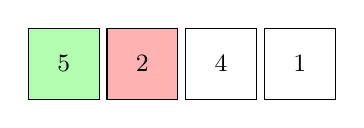
\begin{tikzpicture}
\node[sorted] (c0) at (0,0) {5};
\node[key]    (c1) at (1,0) {2};
\node[unsorted] (c2) at (2,0) {4};
\node[unsorted] (c3) at (3,0) {1};
\end{tikzpicture}
}

\only<2>{
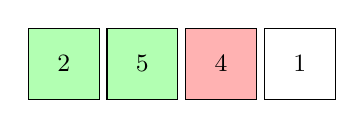
\begin{tikzpicture}
\node[sorted] (c0) at (0,0) {2};
\node[sorted] (c1) at (1,0) {5};
\node[key]    (c2) at (2,0) {4};
\node[unsorted] (c3) at (3,0) {1};
\end{tikzpicture}
}

\only<3>{
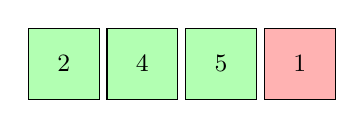
\begin{tikzpicture}
\node[sorted] (c0) at (0,0) {2};
\node[sorted] (c1) at (1,0) {4};
\node[sorted] (c2) at (2,0) {5};
\node[key]    (c3) at (3,0) {1};
\end{tikzpicture}
}

\end{frame}

\begin{frame}{Conclusion}
The green zone grows one position each iteration
\begin{itemize}
  \item This illustrates the invariant used in the correctness proof
  \item Complexity analysis will be discussed with results
\end{itemize}
\end{frame}

\end{document}
